%\documentclass{beamer} %voce pode usar este modelo tambem
\documentclass[t,handout,9pt]{beamer}
\usepackage{graphicx}
\usepackage{url}
\usepackage[british]{babel}
%\batchmode
%\pgfpagesuselayout{4 on 1}[letterpaper,landscape,border shrink=5mm]
\usepackage{amsmath}
\usepackage{amssymb}
\usepackage{amsfonts}
\usepackage{enumerate}
\usepackage{epsfig}
\usepackage{bbm}
\usepackage{calc}
\usepackage{adjustbox}
\usepackage{color}
\usepackage{ifthen}
\usepackage{capt-of}
\usepackage{float}
\usepackage{booktabs}
\usepackage{dcolumn}
\usepackage{multicol}
\usepackage{hyperref}
\usepackage[flushleft]{threeparttable}
\usepackage{subcaption}
\usepackage{adjustbox}
\usepackage{ragged2e}
\usepackage{pgfpages}
%\usepackage{showframe}

\usepackage{cmbright}

\renewcommand\ttdefault{cmvtt} % selects CM typewriter

\usepackage[utf8]{inputenc} % Required for inputting international characters
\usepackage[T1]{fontenc} 	% Output font encoding for international characters

%\DeclareFontShape{OT1}{cmss}{b}{n}{<->ssub * cmss/bx/n}{}

\usetheme[compress]{Berlin}
\definecolor{sapienza}{RGB}{0, 49, 83}
\usecolortheme[named=sapienza]{structure}

\usepackage[backend=bibtex,style=alphabetic,giveninits=true,url=false,eprint=false,doi=false]{biblatex}
\DeclareNameAlias{sortname}{last-first}
\renewcommand*{\nameyeardelim}{\addcomma\addspace}
\renewcommand*{\bibfont}{\footnotesize}
\addbibresource{example.bib}
\setbeamerfont{footnote}{size=\tiny}

\setbeamerfont{title}{size=\LARGE}

% reduce spaces between tables/figures and caption
\usepackage[font=small,skip=1pt]{caption}

%% pgf plots stuff
%\usepackage{pgfplots}
%\pgfplotsset{compat=newest}
%% the following commands are needed for some matlab2tikz features
%\usetikzlibrary{plotmarks}
%\usetikzlibrary{arrows.meta}
%\usepgfplotslibrary{patchplots}

% one navigation dot per slide trick
\AtBeginSection[]{\subsection{}}

% fix misbehave for allowframebreaks
\usepackage{etoolbox}
\makeatletter
\patchcmd{\slideentry}{\ifnum#2>0}{\ifnum2>0}{}% replace the subsection number test with a test that always returns true
% use frame numbers instead of subsection slide numbers so that frames broken over slides get separate circles
\patchcmd{\slideentry}{\c@subsectionslide}{\c@framenumber}{}{\@error{unable to patch}}
\patchcmd{\beamer@writeslidentry}{\c@subsectionslide}{\c@framenumber}{}{\@error{unable to patch}}

% date in footer trick
\makeatletter
  \setbeamertemplate{footline}{%
    \begin{beamercolorbox}[colsep=1.5pt]{upper separation line foot}
    \end{beamercolorbox}
    \begin{beamercolorbox}[ht=2.5ex,dp=1.125ex,%
      leftskip=.3cm,rightskip=.3cm plus1fil]{author in head/foot}%
      \leavevmode{\usebeamerfont{author in head/foot}\insertshortauthor}%
      \hfill%
      {\usebeamerfont{institute in head/foot}\usebeamercolor[fg]{institute in head/foot}\insertshortinstitute}%
    \end{beamercolorbox}%
    \begin{beamercolorbox}[ht=2.5ex,dp=1.125ex,%
      leftskip=.3cm,rightskip=.3cm plus1fil]{title in head/foot}%
      {\usebeamerfont{title in head/foot}\insertshorttitle\hfill\insertshortdate}%
    \end{beamercolorbox}%
    \begin{beamercolorbox}[colsep=1.5pt]{lower separation line foot}
    \end{beamercolorbox}
  }
\makeatletter

% remove dot for titlepage and Outline
\makeatletter
\let\old@beamer@writeslidentry\beamer@writeslidentry
\def\beamer@writeslidentry{%
  \expandafter\beamer@ifempty\expandafter{\beamer@framestartpage}{}% does not happen normally
  {%else
    \clearpage\beamer@notesactions%
  }
}
\makeatother

% let's number figure captions
\setbeamertemplate{caption}[numbered]

% trick for grouping equations
\newenvironment{rcases}
  {\left.\begin{aligned}}
  {\end{aligned}\right\rbrace}

%-------------------------Titulo/Autores/Orientador------------------------------------------------
\title[Introduction to Computer Programming]{Introduction to Computer Programming}
\date[A.Y. 2024-2025]{\\A.Y. 2024-2025}
\author[Alessio Martino]{Prof. Alessio Martino\\
\smallskip
{\small \href{mailto:amartino@luiss.it}{\texttt{amartino@luiss.it}}}\\
\smallskip
}
\institute[10/09/2024]{Department of Business and Management\\Viale Romania 32, 00197 Rome\\[\bigskipamount]

\includegraphics[scale=0.4]{Figures/cliente-luiss.png}%
}

%-------------------------Logo na parte de baixo do slide------------------------------------------
%\pgfdeclareimage[height=0.7cm]{senac-logo}{senac-logo.pdf}
%\logo{\pgfuseimage{senac-logo}\hspace*{0.5cm}}

%-------------------------Este código faz o menuzinho bacana na parte superior do slide------------
%\AtBeginSection[]
%{
%  \begin{frame}<beamer>
%    \frametitle{Outline}
%    \tableofcontents[currentsection]
%  \end{frame}
%}
%\beamerdefaultoverlayspecification{<+->}
% -----------------------------------------------------------------------------

\begin{document}
% -----------------------------------------------------------------------------

%---Gerador de Sumário---------------------------------------------------------

\frame[noframenumbering]{
	\titlepage
}

% begin personalization stuff
\setbeamertemplate{navigation symbols}{%
	\insertslidenavigationsymbol
	\insertframenavigationsymbol
	\insertsubsectionnavigationsymbol
	\insertsectionnavigationsymbol
	\insertdocnavigationsymbol
	\insertbackfindforwardnavigationsymbol
	\hspace{1em}%
	\usebeamerfont{footline}
	\insertframenumber/\inserttotalframenumber%
}
\setbeamertemplate{itemize items}[circle]
\setbeamertemplate{enumerate items}[circle]
\setbeamertemplate{bibliography item}{\insertbiblabel}
% end personalization stuff

\section[]{}
\begin{frame}{Outline}
	\tableofcontents
\end{frame}
%\begin{frame}{Outline}
%\begin{multicols}{2}
%  \tableofcontents
%\end{multicols}
%\end{frame}
%---Fim do Sumário------------------------------------------------------------

% reset navigation dots for other slides
\makeatletter
\let\beamer@writeslidentry\old@beamer@writeslidentry
\makeatother

% -----------------------------------------------------------------------------
\section{Greetings, folks!}
\begin{frame}{Greetings, folks!}
%(Just like you) I'm new here!\\
%\vfill
%\begin{itemize}
%	\item any \textcolor{red}{feedback} is more than welcome!
%\end{itemize}
%\vfill
%Throughout this course ...\\
%\vfill
%\qquad \qquad 	...at any time
%\vfill
%\begin{itemize}
%	\item if you get bored ... \textcolor{red}{ask questions!}
%	\vfill
%	\item if you get lost ... \textcolor{red}{ask questions!}
%	\vfill
%	\item if you'd like to ask questions ... \textcolor{red}{ask questions!}
%\end{itemize}
\vfill
\begin{center}
	Hello students!\\
	Welcome to the \textit{Introduction to Computer Programming} course!
\end{center}
\vfill
\end{frame}
% -----------------------------------------------------------------------------
\section{Web Resources and More}
\begin{frame}{Web Resources and More}
\vfill
You should have access to \textcolor{red}{LUISS Learn}\\
\qquad \url{https://learn.luiss.it/course/view.php?id=23440}\\
(Course website to be set up, I'll add useful info shortly ... I promise)\\
\vfill
\textcolor{red}{Course Syllabus}\\
\url{https://www.luiss.it/cattedreonline/corso/TDS03/0/LAIMBASE/2024}\\
\vfill
\textcolor{red}{Rooms and Timing}\\
\qquad \url{https://pianificazionespazi.luiss.it/PortaleStudentiLuiss}\\
\vfill
\end{frame}
%
\begin{frame}%{Web and Stuff}
\vfill
\textcolor{red}{LUISS Learn} is our e-Learning platform\\
\qquad \url{https://learn.luiss.it/}\\
\vfill
Important that you get access. You'll find there:
\vfill
\begin{itemize}
	\item \textcolor{red}{Slides} and other teaching material
	\vfill
	\item \textcolor{red}{Exercises}
	\vfill
	\item Details on \textcolor{red}{exam} dates, reservations, results\\(besides standard Luiss channels)
	\vfill
	\item \textcolor{red}{Communications} from teacher and teaching assistants
\end{itemize}
\vfill
\end{frame}
%
\begin{frame}
\vfill
\begin{figure}
	
\includegraphics[width=\textwidth]{Figures/LLearn1.png}
\end{figure}
\vfill
\end{frame}
%
\begin{frame}
\vfill
\begin{figure}
	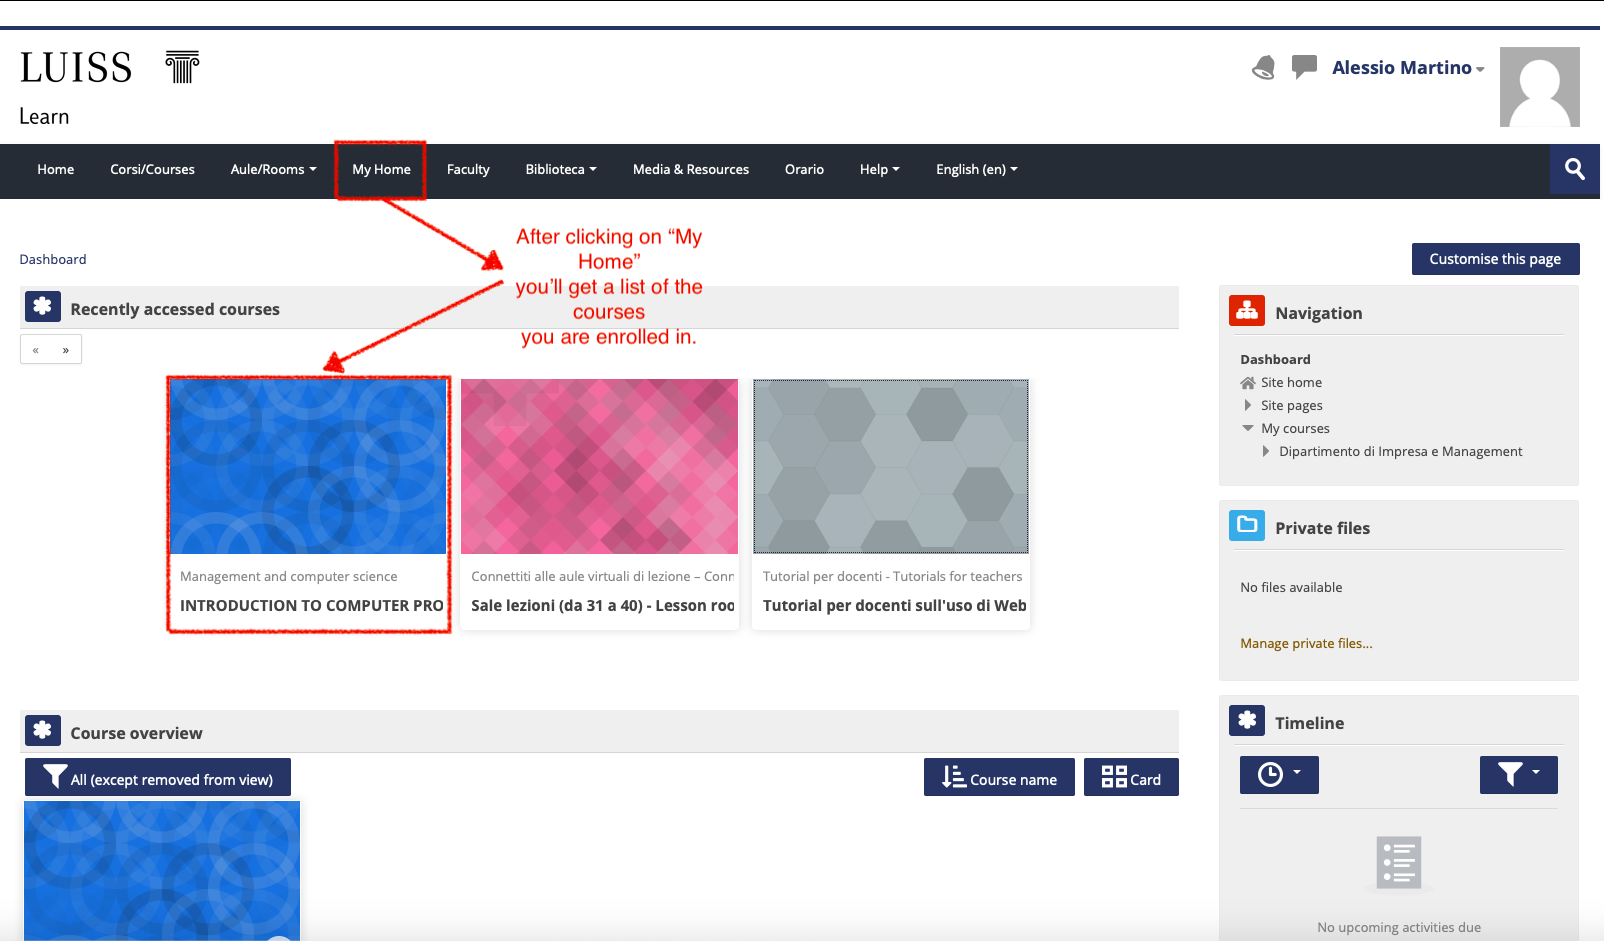
\includegraphics[width=\textwidth]{Figures/LLearn2.png}
\end{figure}
\vfill
\end{frame}
% -----------------------------------------------------------------------------
\section{Personnel}
\begin{frame}{Personnel}
\vfill
Prof. Dr. Alessio Martino\\
\qquad Assistant Professor of Computer Science\\
\qquad \href{mailto:amartino@luiss.it}{\texttt{amartino@luiss.it}}\\
\qquad \textbf{Office Hours}: send me an e-mail so we can arrange a time slot.
\vfill
Dr. Giorgio Piccardo\\
\qquad Teaching Assistant (TA)\\
\qquad \href{mailto:gpiccardo@luiss.it}{\texttt{gpiccardo@luiss.it}}\\
\qquad \textbf{Office Hours}: you can ask info in his first Lab session.
\vfill
Dr. Fabio Angeletti\\
\qquad Teaching Assistant (TA)\\
\qquad \href{mailto:fangeletti@luiss.it}{\texttt{fangeletti@luiss.it}}\\
\qquad \textbf{Office Hours}: you can ask info in his first Lab session.
\vfill
\end{frame}
% -----------------------------------------------------------------------------
\section{Course Info}
\subsection{Course Goals}
\begin{frame}{Course Info}
\vfill
\begin{itemize}
	\item The course is intended to teach \textcolor{red}{basic programming concepts} to students with no prior coding experience, developing an attitude towards \textcolor{red}{computational thinking}
	\vfill
	\item It will provide the students with:
	\begin{itemize}
		\item an understanding of the role that computation can play in solving problems
		\item the ability to write small programs that allow them to accomplish useful goals
	\end{itemize}
\end{itemize}
\vfill
\end{frame}
%
\subsection{Course Roadmap}
\begin{frame}
\vfill
The course will familiarise the students with computer programming and will cover the following topics:
\begin{itemize}
\item Introduction to computation
\item Introduction to programming languages
\item Python basics
\item Variables, data types, expressions
\item Control structures
\item Repetition structures
\item Input / output
\item Functions and modules
\item Recursion
\item Strings
\item Lists
\item Dictionaries
\item Object-oriented programming and classes
\end{itemize}
\vfill
\end{frame}
%
% \subsection{Schedule}
% \begin{frame}
% \vfill
% \begin{figure}
% 	\includegraphics[width=\textwidth]{Figures/Schedule1.png}
% \end{figure}
% \vfill
% \end{frame}
%
%\begin{frame}
%\vfill
%\begin{figure*}
%	\includegraphics[width=\textwidth]{Figures/Schedule2.png}
%\end{figure*}
%\vfill
%\end{frame}
%
\subsection{Organization}
\begin{frame}
\vfill
\begin{itemize}
	\item \textcolor{red}{Lectures} + \textcolor{red}{Lab Sessions}\\
	\qquad \textit{Laptops at your fingertips, always!}
	\vfill
	\item \textcolor{red}{Monday} @ 14:45--16:15\\
	\qquad Several rooms in Viale Romania\\
	\qquad (often) Lab Session with TA
	\vfill
	\item \textcolor{red}{Tuesday} @ 10:00--11:30\\
	\qquad A308 (Viale Romania)\\
	\qquad (often) Theory lectures \& some exercises
	\vfill
	\item \textcolor{red}{Wednesday} @ 15:45--17:15\\
	\qquad A211 (Viale Romania)\\
	\qquad (often) Lab Session with TA
\end{itemize}
\vfill
\end{frame}
%
\subsection{Exams}
\begin{frame}
\vfill
\begin{itemize}
	\item \textcolor{red}{Coding} and \textcolor{red}{Multiple-choice Tests} (70\% of the overall grade -- i.e., 50\% coding and 20\% multiple-choice)
	\item \textcolor{red}{Group project} (30\% of the overall grade)
\end{itemize}
\vfill
In light of the LUISS Continuous Assessment verification method,  we will be having 2 \textit{in itinere} exams:
\begin{itemize}
	\item First Intermediate Test (tentative date: 23/10/2024)
	\item Second Intermediate Test (tentative date: 26/11/2024)
	% \item Checkpoint 3 at Week 10 (tentative date: 15/11/2023)
	% \item Checkpoint 4 at Week 12 (tentative date: 29/11/2023)
\end{itemize}
that replace the \textcolor{red}{Coding test} and the \textcolor{red}{Multiple-choice test}.
\vfill
Students that will not take (or pass) the intermediate tests during the course are required to take the full test at the end of the course.
\vfill
Details on the Group project approx at Week 6.
\vfill
\end{frame}
%
\begin{frame}
\vfill
Each intermediate test is a short exam on the topics covered so far.
\vfill
It will consist of a mixture of coding exercises and theory questions (multiple-choice quiz).
\vfill
Rules (in brief):
\begin{itemize}
	\item the sum of the coding parts between the two tests yields 31
	\item the sum of the theory parts between the two tests yields 31
	\item a score greater than or equal to 16 in each part is enough for successfully passing the coding + theory tests
	% \item each checkpoint is passed if you score above a threshold (to be defined)
	% \item if you fail a checkpoint, you cannot proceed with the next one(s)
\end{itemize}
\vfill
Extra bonus points:
\begin{itemize}
	\item pass the coding + theory test via intermediate tests, you'll get an extra bonus point
	\item if you pass the overall exam (coding + theory + group project) within the Winter session, you'll get an another bonus point
\end{itemize}
\vfill
\end{frame}
% -----------------------------------------------------------------------------
\section{Python, Dear Friend}
\begin{frame}{Python, Dear Friend}
There are just too many ways to use Python in our daily life...
\newline
\adjustbox{valign=t}{\begin{minipage}{0.3\textwidth}
\vspace{1cm}

\includegraphics[width=\textwidth]{Figures/Python1}\vspace{1cm}
Setting up the Python environment ... ?!
\end{minipage}}%
\hfill
\adjustbox{valign=t}{\begin{minipage}[t]{0.5\textwidth}
\vspace{0.5cm}
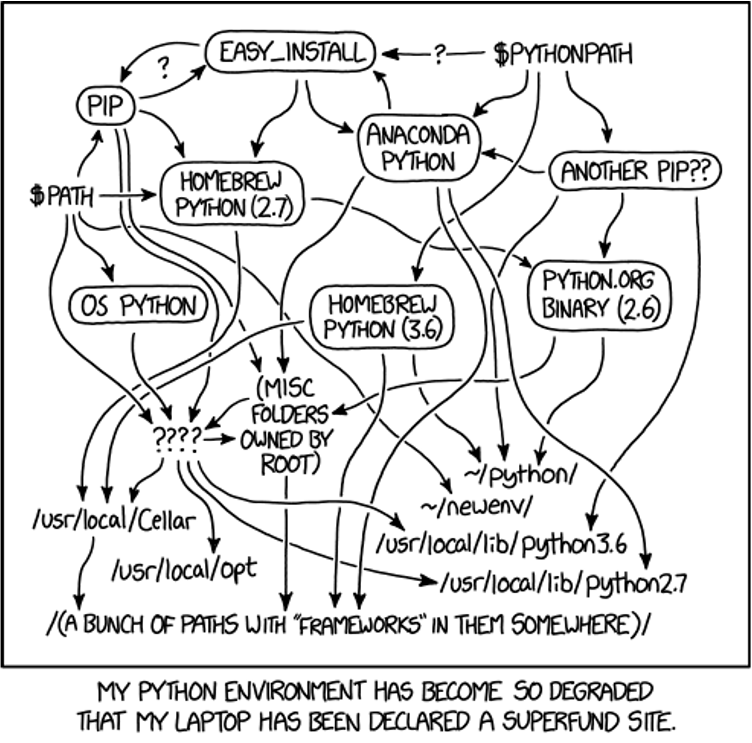
\includegraphics[width=\textwidth]{Figures/Python2}
\end{minipage}}
\end{frame}
%
\begin{frame}
\vfill
We will use Python 3, no Python 2\\
\quad As of January 1\textsuperscript{st}, 2020, Python 2 has been officially discontinued\\
\vfill
Python 3 can be found at\\
\quad \url{https://www.python.org}\\
\vfill
along with its documentation at\\
\quad \url{https://docs.python.org/3/}
\vfill
\begin{itemize}
	\item very rich
	\item very detailed
	\item requires some experience
\end{itemize}
\vfill
\end{frame}
%
\begin{frame}
You can install Python via Anaconda
\begin{figure}
\centering

\includegraphics[width=0.6\textwidth]{Figures/Anaconda1.png}
\end{figure}
% \newline
\adjustbox{valign=t}{\begin{minipage}{0.3\textwidth}
\vspace{0.5cm}
\begin{itemize}
	\item the most popular \textcolor{red}{data science platform}
	\item distribution that includes many many \textcolor{red}{packages}
	\item \textcolor{red}{professional}, with a lot of \textcolor{red}{functionalities}
	\item \textcolor{red}{cross-platform}
	\item \textcolor{red}{free} for individuals
\end{itemize}
\end{minipage}}%
\hfill
\adjustbox{valign=t}{\begin{minipage}[t]{0.5\textwidth}
\vspace{0.5cm}

\includegraphics[width=\textwidth]{Figures/Anaconda2}
\end{minipage}}
\end{frame}
%
\begin{frame}
\vfill
Some Anaconda resources:\\
\begin{itemize}
\item Official website \& download:\\
\quad \url{https://www.anaconda.com/}\\
\item Documentation:\\
\quad \url{https://docs.anaconda.com/anaconda/}\\
\item Installation guide:\\
\quad \url{https://docs.anaconda.com/anaconda/install/}\\
\item Community:\\
\quad \url{https://anaconda.org}\\
\item Anaconda Navigator:\\
\quad \url{https://docs.anaconda.com/anaconda/navigator/}\\
\end{itemize}
\vfill
ToDo:\\
$\rightarrow$ Try to install Python/Anaconda before the next lab session!\\
You can get help from the TA, should you have any issues.
\vfill
\end{frame}
%
\begin{frame}
Like Virgil with Dante, Anaconda Navigator guides you through
\vfill
\begin{figure}
\centering
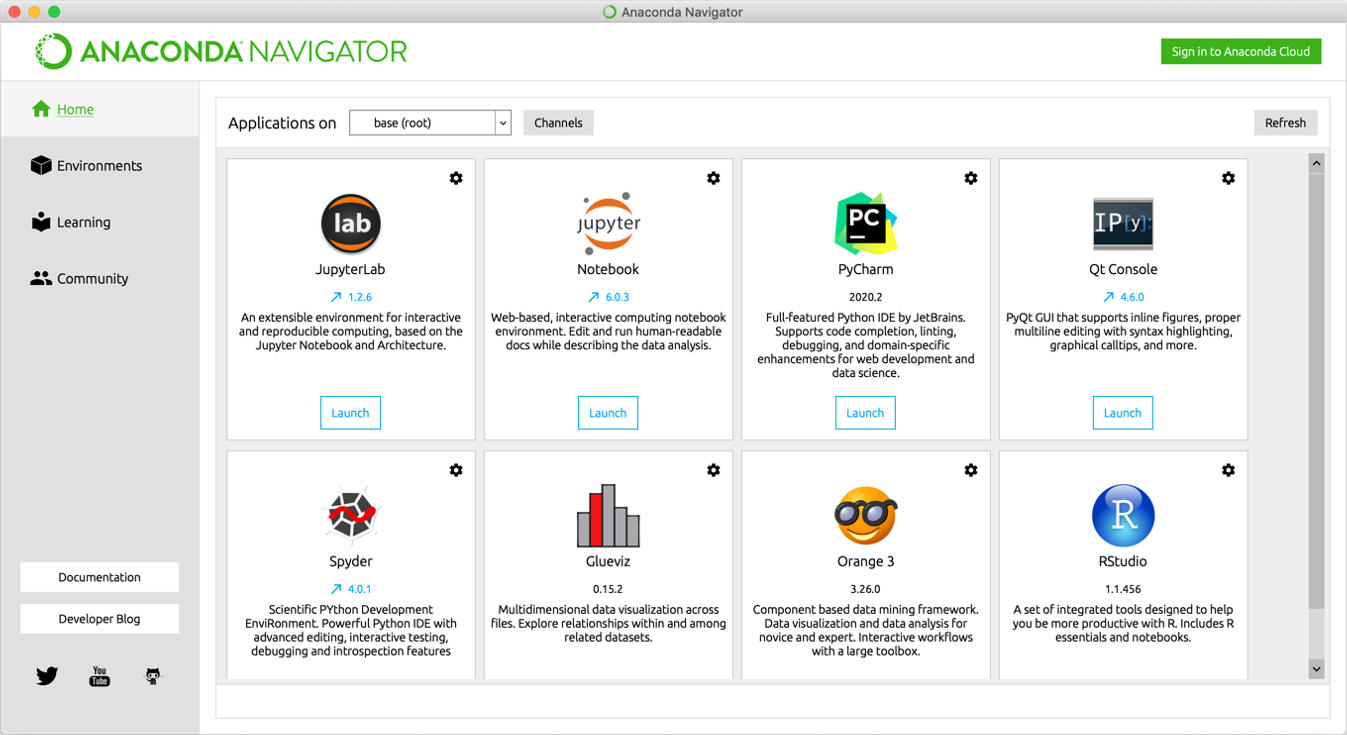
\includegraphics[width=\textwidth]{Figures/Anaconda3.png}
\end{figure}
\end{frame}
%
\begin{frame}
\vfill
A full in-browser alternative: PythonAnywhere\\
\quad \url{https://eu.pythonanywhere.com/}\\
\vfill
\begin{itemize}
	\item Work in Python from a browser
	\item Support both interactive and script mode (files)
	\item Need to create an account\\
	$\rightarrow$ A free account is more than enough for this course
	\item Good tutorial by Allen Downey\\
	$\rightarrow$ \url{http://www.allendowney.com/wp/books/think-python-2e/}
\end{itemize}
\vfill
\end{frame}
%
\begin{frame}
\vfill
A shoulder to cry on if your code doesn't work: Python Tutor\\
\quad \url{http://pythontutor.com/}\\
\vfill
\begin{itemize}
	\item Observe content of variables
	\item Observe single execution steps
	\item Go forward and backwards, even step-by-step
\end{itemize}
\vfill
\begin{figure}
\centering
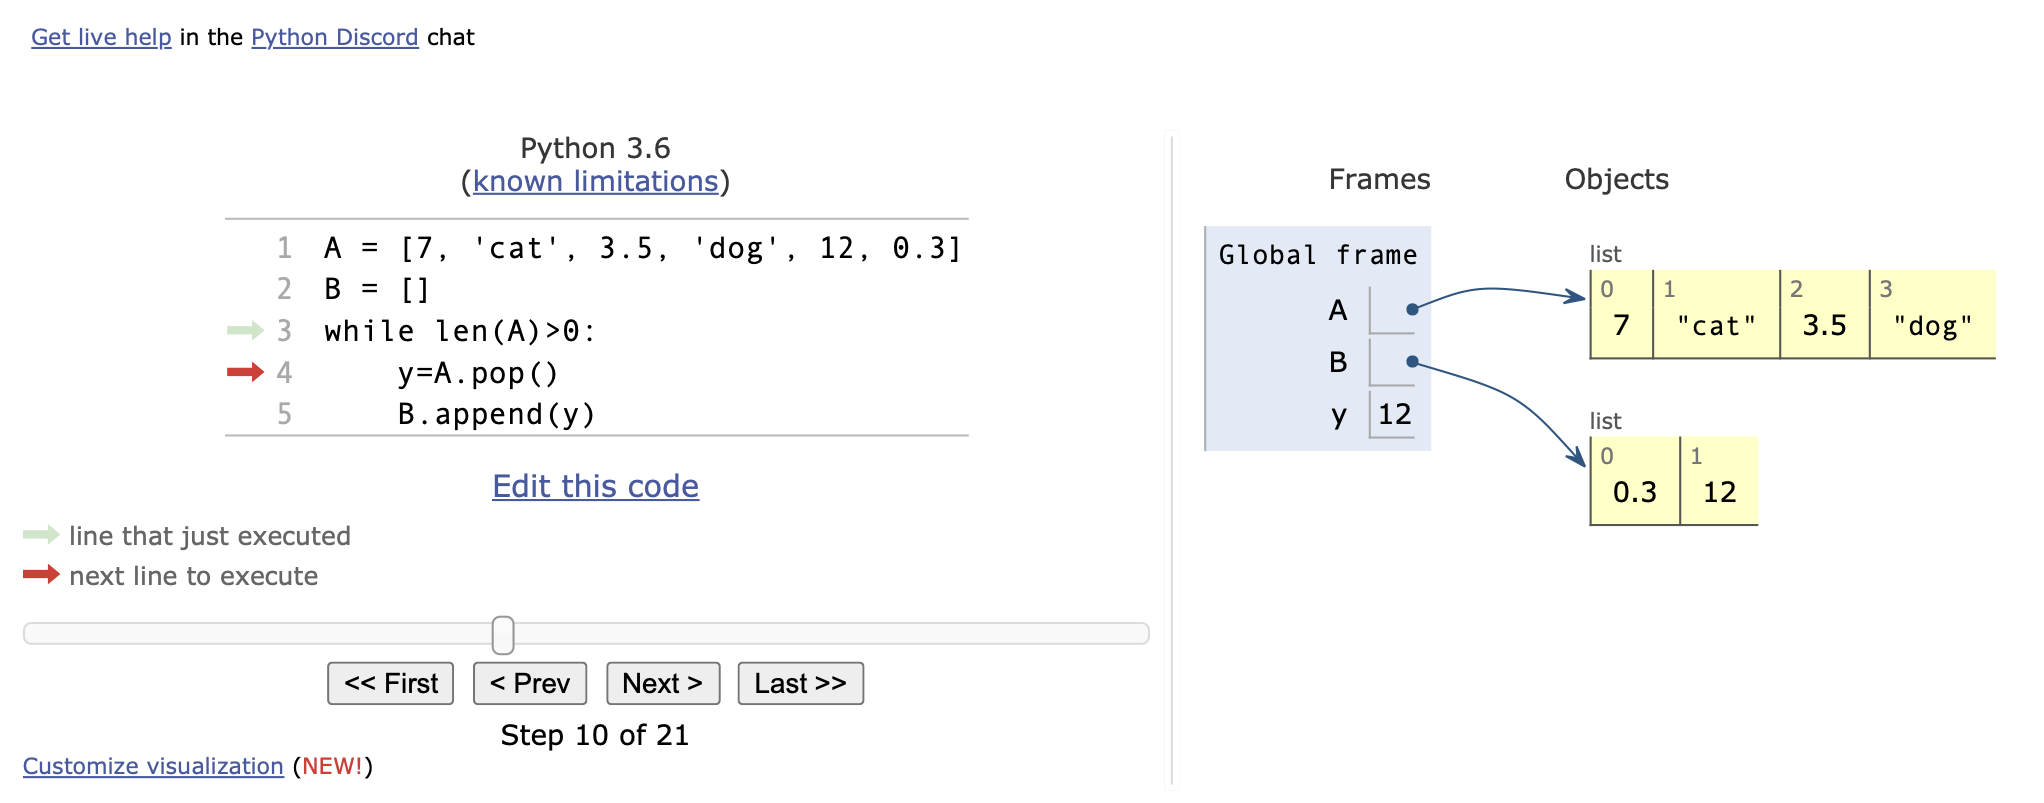
\includegraphics[width=\textwidth]{Figures/PythonTutor.png}
\end{figure}
\end{frame}
% -----------------------------------------------------------------------------
%\section{Introduction}
%\begin{frame}{Introduction}
%Pattern Recognition and Machine Learning are well-established fields when it comes to deal with metric (Euclidean) input spaces:\\
%$\qquad\rightarrow$ patterns are described by real-valued feature vectors\\
%\medskip
%However, when dealing with real-world complex systems, non-conventional data structures are more suited, such as
%\begin{itemize}
%	\item graphs\\
%		$\rightarrow$ possibly labelled on nodes and/or edges
%	\item sequences\\
%		$\rightarrow$ of objects or events
%	\item images
%	\item videos
%	\item text documents
%	\item time series.
%\end{itemize}
%\end{frame}
%
%\begin{frame}
%A plethora of application fields:
%\begin{itemize}
%	\item biology
%	\item (cyber)security
%	\item text mining and sentiment analysis
%	\item image analysis.
%\end{itemize}
%\medskip
%However, structured data might lie in a \textit{non-metric} space.\\
%\medskip
%In short, an input space $\mathcal{X}$ is said to be \textit{non-metric} if, given a measure of dissimilarity $d(\cdot,\cdot):\mathcal{X}\times\mathcal{X}\rightarrow\mathbb{R}$, at least one of the following properties does not hold \parencite{Martino2018,pkekalska2005dissimilarity}:
%\begin{itemize}
%	\item symmetry
%	\item identity
%	\item triangle inequality
%	\item non-negativity.
%\end{itemize}
%\end{frame}
%
%\begin{frame}
%Scope of this talk:
%\vfill
%\begin{itemize}
%	\item further bridging the gap on structural pattern recognition\\
%		$\rightarrow$ five pattern recognition techniques\\
%		$\rightarrow$ emphasis on graphs and hypergraphs
%	\vfill
%	\item grey-box models\\
%		$\rightarrow$ interpretable by field-experts
%	\vfill
%	\item real-world biological case studies:
%		\begin{enumerate}
%		\item modelling structure-vs-function relationship in protein networks
%		\item modelling structure-vs-solubility relationship in protein networks
%		\item analysis of metabolic pathways.
%		\end{enumerate}
%	\vfill
%	\item assessment against state-of-the-art approaches\\
%		$\rightarrow$ on freely-available benchmark datasets.
%\end{itemize}
%\end{frame}
% -----------------------------------------------------------------------------
%\section{Current Approaches}
%\begin{frame}{Current Approaches}
%Current strategies for dealing with structured data can be broadly divided in three main families \parencite{Martino2018}:
%\begin{enumerate}
%	\item feature generation and feature engineering\\\medskip
%	\item ad-hoc dissimilarities in the input spaces\\\medskip
%	\item embedding techniques\\\medskip
%	\begin{enumerate}
%		\item dissimilarity spaces\\\medskip
%		\item kernel methods\\\medskip
%		\item information granulation\\\medskip
%		\item neural approaches\\\medskip
%	\end{enumerate}
%\end{enumerate}
%\medskip
%... but also hybridisations exist.
%\end{frame}
%
%\subsection{Feature Generation and Feature Engineering}
%\begin{frame}
%Define a problem-related (input space-related) mapping function
%\begin{equation*}
%m:\mathcal{X}\rightarrow\mathbb{R}^n
%\end{equation*}
%Move the problem (cast the dataset) towards the Euclidean space.\\
%\medskip
%The Euclidean space is obviously metric and any pattern recognition and computational intelligence algorithm can be used without alterations.\\
%\vfill
%\begin{block}{Note}
%Defining $m(\cdot)$ might not be trivial and requires some a-priori knowledge on the input space and/or the problem at hand.
%\end{block}
%\vfill
%Specific subsets of numerical features which can be drawn from structured data are suitable for solving specific problems.
%\end{frame}
%
%\subsection{Ad-hoc Dissimilarities in the Input Space}
%\begin{frame}
%Use dissimilarity functions tailored for the input-space at hand, such as:
%\begin{itemize}
%\item edit distances for graphs \parencite{Livi2013}
%\item edit distances for sequences \parencite{levenshtein1966binary}
%\item dynamic time warping \parencite{sakoe1978dynamic}
%\end{itemize}
%without moving the problem towards any Euclidean space.\\
%\vfill
%\begin{block}{Note}
%Not all algorithms do work directly in structured domains. They must rely on pairwise dissimilarities only and avoid algebraic structures and operators such as mean, median or inner product.
%\end{block}
%\vfill
%Good classification algorithms:
%\begin{itemize}
%	\item $K$-Nearest Neighbours
%	\item (kernelised) Support Vector Machines.
%\end{itemize}
%Good clustering algorithms:
%\begin{itemize}
%	\item BSAS
%	\item $k$-medoids
%	\item DB-SCAN
%	\item hierarchical/linkage.
%\end{itemize}
%\end{frame}
%
%\subsection{Dissimilarity Spaces}
%\begin{frame}
%Express each pattern from the dataset $\mathcal{D}$ according to the distances with respect to all other patterns, including itself \parencite{pkekalska2005dissimilarity}.\\
%Build the full dissimilarity matrix $\mathbf{D}$ such that
%\begin{equation*}
%\mathbf{D}_{i,j} = d(x_i,x_j) \quad \forall i,j=1,\ldots,\arrowvert\mathcal{D}\arrowvert
%\end{equation*}
%Since $\mathbf{D}\in\mathbb{R}^{\arrowvert\mathcal{D}\arrowvert\times\arrowvert\mathcal{D}\arrowvert}$, it can be seen as lying in a metric space: use the $i$\textsuperscript{th} row from $\mathbf{D}$ in lieu of the the $i$\textsuperscript{th} pattern from $\mathcal{D}$.\\
%\vfill
%\begin{block}{Note}
%The dissimilarity measure $d(\cdot,\cdot)$ must be custom.\\
%Not suitable for big datasets since building $\mathbf{D}$ requires $\mathcal{O}(\arrowvert\mathcal{D}\arrowvert^2)$, but a subset $\mathcal{R}\subset\mathcal{D}$ of representative patterns can be selected and $\mathbf{D}\in\mathbb{R}^{\arrowvert\mathcal{D}\arrowvert\times\arrowvert\mathcal{R}\arrowvert}$ \parencite{pkekalska2006prototype}.
%\end{block}
%\vfill
%Suitable strategies for choosing $\mathcal{R}$:
%\begin{itemize}
%	\item random selection
%	\item pre-clustering
%	\item optimisation-driven.
%\end{itemize}
%\end{frame}
%
%\subsection{Kernel Methods}
%\begin{frame}
%Kernel methods perform an implicit embedding towards a (possibly) infinite-dimensional Hilbert space in which linear separation is more likely.\\
%\medskip
%A PSD-kernel matrix encodes pairwise similarities between data, either be in a vector form:
%\begin{itemize}
%	\item dot product
%	\item radial basis function, polynomial, Laplacian, ...
%\end{itemize}
%or in a non-conventional form
%\begin{itemize}
%	\item string kernels \parencite{Leslie,10.1093/bioinformatics/btg431}\\
%		$\rightarrow$ spectrum, mismatch, substring, ...
%	\item graph kernels \parencite{GHOSH201888}\\
%		$\rightarrow$ tree, random walks, paths, cycles, propagation, diffusion, ...
%	\item image kernels\\
%		$\rightarrow$ texture, HOG, color channels, ...
%\end{itemize}
%and can be fed to a kernelised classifier such as Support Vector Machine.
%\end{frame}
%
%\subsection{Information Granulation}
%\begin{frame}
%Another explicit embedding procedure that relies on \textit{information granules} (groups of data with functional and/or structural similarity).\\
%\medskip
%Information granules can be intended as meaningful and recurring sub-structures pivotal for the embedding procedure.\\
%\medskip
%The embedding relies on the so-called \textit{symbolic histograms}: for a given structured pattern $x\in\mathcal{X}$ and for a given set of information granules $\mathcal{A}$, one gets
%\begin{equation*}
%	\mathbf{h}_x(\mathcal{A}) = [\text{count}(\mathcal{A}_1,x), \ldots, \text{count}(\mathcal{A}_M,x)]
%\end{equation*}
%\vfill
%\begin{block}{Note}
%The data-driven synthesis of $\mathcal{A}$ is crucial: the set of information granules must fill the semantic gap between the two domains.
%\end{block}
%\vfill Desiderata:
%\begin{itemize}
%	\item symbols in $\mathcal{A}$ must be informative
%	\item $\mathcal{A}$ should have low cardinality\\
%		$\rightarrow$ low embedding complexity\\
%		$\rightarrow$ easy interpretation by field-experts
%\end{itemize}
%\end{frame}
%
%\subsection{Neural Approaches}
%\begin{frame}
%Rely on the power of artificial neural networks in order to build the embedding space in an automatic and data-driven way \parencite{Wu_2021}.\\
%\medskip
%Exploit the concept of neighbourhoods (i.e., message passing amongst nodes):
%\begin{itemize}
%	\item spatial convolution
%	\item spectral convolution
%	\item recurrent convolution
%\end{itemize}
%\medskip
%Capable of learning the embedding at node level or graph level:
%\begin{itemize}
%	\item graph classification
%	\begin{itemize}
%		\item classify the whole graph into different categories
%	\end{itemize}
%	\item node classification
%	\begin{itemize}
%		\item predict the node embedding for every node in a graph
%	\end{itemize}
%	\item link prediction
%	\begin{itemize}
%		\item predict if two entities have a connection in-between
%	\end{itemize}
%\end{itemize}
%\end{frame}
% -----------------------------------------------------------------------------
%\section{Research Activities}
%\subsection{Graph Classification by Spectral Density Estimation}
%\begin{frame}{Research Activities}
%Goal: describe a graph by means of its spectral density \parencite{Martino2017,maiorino2017spectral}.\\
%\vfill
%A graph $\mathcal{G}=(\mathcal{V},\mathcal{E})$ with $n=\arrowvert\mathcal{V}\arrowvert$ nodes can be described by the following matrices:
%\begin{itemize}
%	\item adjacency matrix $\mathbf{A}\in\mathbb{R}^{n \times n}$
%	\item degree matrix $\mathbf{D}\in\mathbb{R}^{n \times n}$
%	\item Laplacian matrix $\mathbf{L} = \mathbf{D}-\mathbf{A}$
%	\item normalised Laplacian matrix $\overline{\mathbf{L}} = \mathbf{D}^{-\frac{1}{2}}\mathbf{L}\mathbf{D}^{-\frac{1}{2}}$
%\end{itemize}
%\vfill
%\begin{block}{Problem}
%$\mathbf{A}$, $\mathbf{D}$, $\mathbf{L}$, $\overline{\mathbf{L}}\in\mathbb{R}^{n \times n}$: impossible to compare graphs having different number of nodes.
%\end{block}
%\end{frame}
%
%\begin{frame}
%The normalised Laplacian has the following intriguing property:\\
%$\qquad\rightarrow$ its \textit{spectrum} lies in $[0,2]$ regardless of $\mathcal{G}$\\
%So let us consider the spectral decomposition of $\overline{\mathbf{L}}$
%\begin{equation}
%	\overline{\mathbf{L}} = \mathbf{V} \bm{\Lambda} \mathbf{V}^T
%\end{equation}
%where $\bm{\Lambda} = \text{diag}(\{\lambda_1,\ldots,\lambda_n\})$.
%\begin{block}{Problem}
%The size of the spectrum equals the number of nodes: it cannot be used to compare graphs having different sizes.
%\end{block}
%Estimate the spectral density of $\overline{\mathbf{L}}$ by means of a kernel density estimator:
%\begin{equation}
%	p(x)=\dfrac{1}{n}\sum\nolimits_{i=1}^{n}\dfrac{1}{\sqrt{2\pi\sigma^2}}\text{exp}\left\{\dfrac{-(x-\lambda_i)^2}{2\sigma^2}\right\}
%\end{equation}
%For two graphs $\mathcal{G}_a$ and $\mathcal{G}_b$ one gets $p_a(x)$ and $p_b(x)$. Their distance reads as
%\begin{equation}
%	d(\mathcal{G}_a,\mathcal{G}_b)=\int_{0}^{2}(p_a(x)-p_b(x))^2 dx
%	\label{eq:graphdiff}
%\end{equation}
%or, in the discrete domain, by sampling a finite number of $m$ points from $p(x)$.% and the latter collapses into the Euclidean distance.
%\end{frame}
%
%\begin{frame}
%\begin{figure}
%     \centering
%     \begin{subfigure}[b]{0.3\textwidth}
%         \centering
%         \includegraphics[width=\textwidth]{Figures/SpectralDensity_stepbystep_01_randomgraph}
%         \caption{A graph $\mathcal{G}$}
%     \end{subfigure}
%     \hfill
%     \begin{subfigure}[b]{0.3\textwidth}
%         \centering
%         \includegraphics[width=\textwidth]{Figures/SpectralDensity_stepbystep_02_adjacency}
%         \caption{Adjacency Matrix $\mathbf{A}$}
%     \end{subfigure}
%     \hfill
%     \begin{subfigure}[b]{0.3\textwidth}
%         \centering
%         \includegraphics[width=\textwidth]{Figures/SpectralDensity_stepbystep_03_degree}
%         \caption{Degree Matrix $\mathbf{D}$}
%     \end{subfigure}
%     \vfill
%     \begin{subfigure}[b]{0.3\textwidth}
%         \centering
%         \includegraphics[width=\textwidth]{Figures/SpectralDensity_stepbystep_04_laplacian}
%         \caption{Laplacian Matrix $\mathbf{L}$}
%     \end{subfigure}
%     \hfill
%     \begin{subfigure}[b]{0.3\textwidth}
%         \centering
%         \includegraphics[width=\textwidth]{Figures/SpectralDensity_stepbystep_05_normlaplacian}
%         \caption{Normalised Laplacian $\overline{\mathbf{L}}$}
%     \end{subfigure}
%     \hfill
%     \begin{subfigure}[b]{0.3\textwidth}
%         \centering
%         \includegraphics[width=\textwidth]{Figures/SpectralDensity_stepbystep_06_spectraldensity}
%         \caption{Spectral Density}
%     \end{subfigure}
%\vfill
%\caption{Feature Generation Pipeline}
%\end{figure}
%\end{frame}
%
%\subsection{Graph Classification using the Betti Numbers Sequence}
%\begin{frame}
%Goal: describe a graph by the sequence of its Betti numbers \parencite{8489307}.\\
%\medskip
%The Betti numbers are invariant descriptors of a topological space and can be evaluated starting from a point cloud $\mathcal{C}\equiv\mathcal{V}$ equipped with a notion of distance $d(\cdot,\cdot)$.\\
%\medskip
%The topological space shall be described by means of its \textit{simplices} drawn from a properly-constructed \textit{simplicial complex}.\\
%\medskip
%\begin{block}{Definition \parencite{carlsson2009topology,zomorodian2012topological,doi:10.1146/annurev-statistics-031017-100045}}
%A simplicial complex is a finite collection of simplices (points, lines, tetrahedrons and higher-order analogues) which is closed to the inclusion of the faces.
%\end{block}
%\begin{block}{Definition \parencite{ZOMORODIAN2010263}}
%The Vietoris-Rips complex is a simplicial complex obtained by forming a $k$-simplex for every finite set of $k+1$ points whose pairwise distances are at most $\epsilon$.
%\end{block}
%\end{frame}
%
%\begin{frame}
%\begin{figure}
%     \centering
%     \begin{subfigure}[b]{0.3\textwidth}
%         \centering
%         \includegraphics[width=\textwidth]{Figures/PCN_VRcomplex_eps4}
%         \caption{$\epsilon=4$}
%     \end{subfigure}
%     \hfill
%     \begin{subfigure}[b]{0.3\textwidth}
%         \centering
%         \includegraphics[width=\textwidth]{Figures/PCN_VRcomplex_eps5}
%         \caption{$\epsilon=5$}
%     \end{subfigure}
%     \hfill
%     \begin{subfigure}[b]{0.3\textwidth}
%         \centering
%         \includegraphics[width=\textwidth]{Figures/PCN_VRcomplex_eps6}
%         \caption{$\epsilon=6$}
%     \end{subfigure}
%     \vfill
%     \begin{subfigure}[b]{0.3\textwidth}
%         \centering
%         \includegraphics[width=\textwidth]{Figures/PCN_VRcomplex_eps7}
%         \caption{$\epsilon=7$}
%     \end{subfigure}
% 	\
%     \begin{subfigure}[b]{0.3\textwidth}
%         \centering
%         \includegraphics[width=\textwidth]{Figures/PCN_VRcomplex_eps8}
%         \caption{$\epsilon=8$}
%     \end{subfigure}
%\vfill
%\caption{Topological configuration of a sample PCN (PDB 1HNR) at different scales.}
%\end{figure}
%\end{frame}
%
%\begin{frame}
%%\begin{block}{Definition}
%%The Vietoris-Rips complex is a simplicial complex obtained by forming a $k$-simplex for every finite set of $k-1$ points whose pairwise distances are at most $\epsilon$.
%%\end{block}
%Given a simplicial complex $\mathcal{S}$, its Betti numbers can be evaluated by considering the boundary operator $\partial_k:\mathcal{S}^{(k)}\rightarrow\mathcal{S}^{(k-1)}$. The $k$-order \textit{homology group} is defined as
%%
%\begin{equation}
%	\mathcal{H}_k = \text{ker}\{ \partial_k \}/\text{im}\{ \partial_{k+1} \}
%	\label{eqn:betti_1}
%\end{equation}
%%
%The rank of $\mathcal{H}_k$, namely the $k$\textsuperscript{th} Betti number $\beta_k$, reads as
%%
%\begin{align}
%\begin{split}
%	\beta_k & = \text{rank}\{ \text{ker}\{ \partial_k \} \} - \text{rank} \{ \text{im}\{ \partial_{k+1} \} \} = \\
%	& = \left( \text{card}\{\partial_k\}-\text{rank}\{ \text{im} \{ \partial_k \} \} \right) - \text{rank}\{ \text{im} \{ \partial_{k+1} \} \}
%	\label{eqn:betti_2}
%\end{split}
%\end{align}
%The Betti numbers have the following properties:
%\begin{enumerate}
%	\item they are all finite and vanish after the spatial dimension
%	\item the $0$\textsuperscript{th} Betti number corresponds to the number of connected components%(0-dimensional holes)
%	\item the $1$\textsuperscript{st} Betti number corresponds to the number of circular holes%(1-dimensional holes)
%	\item the $2$\textsuperscript{nd} Betti number corresponds to the number of voids/cavities%(2-dimensional holes).
%\end{enumerate}
%So, each point cloud lying in an $m$-dimensional space and analysed thanks to $j$ candidate threshold values can be cast towards the following vector
%\begin{equation}
%	\left[ \beta_0^{(\epsilon_1)},\ldots, \beta_{m-1}^{(\epsilon_1)},\ldots, \beta_0^{(\epsilon_j)},\ldots, \beta_{m-1}^{(\epsilon_j)}\right]
%	\label{eq:bettivector}
%\end{equation}
%\end{frame}
%
%\begin{frame}
%\vfill
%\begin{figure}
%     \centering
%     \begin{subfigure}[b]{0.45\textwidth}
%         \centering
%         \includegraphics[width=\textwidth]{Figures/bettinumbers_028_18_32}
%         \caption{$\mathcal{S}_1$}
%     \end{subfigure}
%     \
%     \begin{subfigure}[b]{0.45\textwidth}
%         \centering
%         \includegraphics[width=\textwidth]{Figures/bettinumbers_0302_42_41}
%         \caption{$\mathcal{S}_2$}
%     \end{subfigure}
%\caption{Example of Simplicial Complexes and their Homology.}
%\end{figure}
%\vfill
%\end{frame}
%
%\subsection{Embedding over Simplicial Complexes}
%\begin{frame}
%Goal: address whether simplices can be interpreted as information granules \parencite{Martino_ALGO_submitted}.\\
%\medskip
%Let $\mathcal{D}_\text{TR}$, $\mathcal{D}_\text{VAL}$ and $\mathcal{D}_\text{TS}$ be three non-overlapping sets of a node-labelled dataset.\\
%\medskip
%The alphabet synthesis procedure works as follows:
%\begin{enumerate}
%	\item infer the simplicial complex from all items in $\mathcal{D}_\text{TR}$, $\mathcal{D}_\text{VAL}$ and $\mathcal{D}_\text{TS}$
%	\item map each vertex according to its label
%	\item consider $\mathcal{A}$ as the set of unique simplices in $\mathcal{D}_\text{TR} \cup \mathcal{D}_\text{VAL}$
%\end{enumerate}
%\medskip
%The embedding follows the symbolic histogram approach:
%\begin{itemize}
%	\item $\mathbf{D}_\text{TR} \in \mathbb{R}^{\arrowvert\mathcal{D}_\text{TR}\arrowvert\times\arrowvert\mathcal{A}\arrowvert}$
%	\item $\mathbf{D}_\text{VAL} \in \mathbb{R}^{\arrowvert\mathcal{D}_\text{VAL}\arrowvert\times\arrowvert\mathcal{A}\arrowvert}$
%\end{itemize}
%\medskip
%An optimisation stage aims at selecting a suitable subset of symbols from $\mathcal{A}$ in order to maximise performances.
%\end{frame}
%
%\begin{frame}
%%A genetic algorithm aims at selecting a suitable subset of symbols from $\mathcal{A}$ in order to maximise performances.\\
%%\medskip
%The search space reads as
%\begin{equation}
%	[\mathcal{H} \quad \mathbf{w}]
%\end{equation}
%where
%\begin{itemize}
%	\item $\mathcal{H}$ regards the classifier hyperparameters
%	\item $\mathbf{w}\in \{0,1\}^{\arrowvert\mathcal{A}\arrowvert}$ selects suitable alphabet symbols for the embedding.
%\end{itemize}
%%$\mathcal{H}$ regards the classifier hyperparameters and $\mathbf{w}\in \{0,1\}^{\arrowvert\mathcal{A}\arrowvert}$ selects suitable alphabet symbols for the embedding.\\
%\medskip
%The objective function reads as
%\begin{equation}
%	F = (1-\alpha) \cdot P + \alpha \cdot C
%\label{eqn:fitness}
%\end{equation}
%where
%\begin{itemize}
%	\item $P$ considers the classifier performances (e.g., accuracy, informedness)
%	\item $C$ accounts the complexity of the embedding space (\% selected symbols).
%\end{itemize}
%%$P$ considers the classifier performances and $C$ accounts the complexity of the embedding space.\\
%\medskip
%As the optimisation ends, one gets
%\begin{itemize}
%	\item $\mathcal{H}^\star$
%	\item $\mathbf{w}^\star\rightarrow\mathcal{A}^\star$.
%\end{itemize}
%\medskip
%The final performances are evaluated on $\mathbf{D}_\text{TS} \in \mathbb{R}^{\arrowvert\mathcal{D}_\text{TS}\arrowvert\times\arrowvert\mathcal{A}^\star\arrowvert}$
%\end{frame}
%
%\begin{frame}
%\vfill
%\begin{figure}
%     \centering
%         \includegraphics[width=\textwidth]{Figures/block diagrams-Page-2}
%\caption{Embedding over Simplicial Complexes: summary of the model training.}
%\end{figure}
%\vfill
%\end{frame}
%
%\begin{frame}
%\vfill
%\begin{figure}
%     \centering
%         \includegraphics[width=\textwidth]{Figures/SH}
%\caption{Example of Embedding via Symbolic Histograms.}
%\end{figure}
%\vfill
%\end{frame}
%
%\subsection{Embedding via INDVAL}
%\begin{frame}
%Goal: statistically relevant network motifs as information granules \parencite{Martino_CBAC_submitted, martino2019universal,martinoAccess}.\\
%\vfill
%Let $\mathcal{D}_\text{TR}$, $\mathcal{D}_\text{VAL}$ and $\mathcal{D}_\text{TS}$ be three non-overlapping sets of a fully-labelled dataset.\\
%\vfill
%The INDVAL score for the $i$\textsuperscript{th} subgraph for the $j$\textsuperscript{th} class is defined as:
%\begin{equation}
%A_{i,j} = \frac{\text{\# patterns in class }j \text{ having subgraph }i}{\text{\# patterns having subgraph }i}
%\label{eq:A}
%\end{equation}
%\begin{equation}
%B_{i,j} = \frac{\text{\# patterns in class }j \text{ having subgraph }i}{\text{\# patterns belonging to class }j}
%\label{eq:B}
%\end{equation}
%\begin{equation}
%I_{i,j} = A_{i,j} \cdot B_{i,j} \cdot 100
%\label{eq:INDVAL}
%\end{equation}\\
%\vfill
%The end-user defines a threshold $T\in(0,100)$ and all subgraphs having $I\geq T$ for any $j$ compose the alphabet $\mathcal{A}$.
%\end{frame}
%
%\begin{frame}
%\begin{figure}
%     \centering
%     \subfloat[class 1]{\includegraphics[width=0.25\textwidth]{Figures/G1_class1.png}}
%     \subfloat[class 1]{\includegraphics[width=0.25\textwidth]{Figures/G2_class1.png}}
%     \subfloat[class 2]{\includegraphics[width=0.25\textwidth]{Figures/G1_class2.png}}
%     \subfloat[class 2]{\includegraphics[width=0.25\textwidth]{Figures/G2_class2.png}}
%     \caption{The idea behind the INDVAL score: a toy dataset}
%\end{figure}
%\textcolor{green}{$A_{\text{A-B}}^{(1)} = 2/2$ \qquad\qquad $B_{\text{A-B}}^{(1)} = 2/2$ \qquad\qquad $I_{\text{A-B}}^{(1)} = 1 \cdot 1 \cdot 100 = 100$\\
%$A_{\text{A-B}}^{(2)} = 0/2$ \qquad\qquad $B_{\text{A-B}}^{(2)} = 0/2$ \qquad\qquad $I_{\text{A-B}}^{(2)} = 0 \cdot 0 \cdot 100 = 0$\\}
%
%$A_{\text{B-D}}^{(1)} = 1/3$ \qquad\qquad $B_{\text{B-D}}^{(1)} = 1/2$ \qquad\qquad $I_{\text{B-D}}^{(1)} = 0.3 \cdot 0.5 \cdot 100 = 15$\\
%$A_{\text{B-D}}^{(2)} = 2/3$ \qquad\qquad $B_{\text{B-D}}^{(2)} = 2/2$ \qquad\qquad $I_{\text{B-D}}^{(2)} = 0.6 \cdot 1 \cdot 100 = 60$\\
%
%$A_{\text{B-C}}^{(1)} = 0/1$ \qquad\qquad $B_{\text{B-C}}^{(1)} = 0/2$ \qquad\qquad $I_{\text{B-C}}^{(1)} = 0 \cdot 0 \cdot 100 = 0$\\
%$A_{\text{B-C}}^{(2)} = 1/1$ \qquad\qquad $B_{\text{B-C}}^{(2)} = 1/2$ \qquad\qquad $I_{\text{B-C}}^{(2)} = 1 \cdot 0.5 \cdot 100 = 50$\\
%
%\textcolor{red}{$A_{\text{C-D}}^{(1)} = 1/2$ \qquad\qquad $B_{\text{C-D}}^{(1)} = 1/2$ \qquad\qquad $I_{\text{C-D}}^{(1)} = 0.5 \cdot 0.5 \cdot 100 = 25$\\
%$A_{\text{C-D}}^{(2)} = 1/2$ \qquad\qquad $B_{\text{C-D}}^{(2)} = 1/2$ \qquad\qquad $I_{\text{C-D}}^{(2)} = 0.5 \cdot 0.5 \cdot 100 = 25$\\}
%
%\textcolor{red}{$A_{\text{A-C}}^{(1)} = 2/4$ \qquad\qquad $B_{\text{A-C}}^{(1)} = 2/2$ \qquad\qquad $I_{\text{A-C}}^{(1)} = 0.5 \cdot 1 \cdot 100 = 50$\\
%$A_{\text{A-C}}^{(2)} = 2/4$ \qquad\qquad $B_{\text{A-C}}^{(2)} = 2/2$ \qquad\qquad $I_{\text{A-C}}^{(2)} = 0.5 \cdot 1 \cdot 100 = 50$}
%\end{frame}
%
%\begin{frame}
%Let us complicate the problem: the dataset is fully labelled.
%\vfill
%We define a Graph Edit Distance $d:\mathcal{G}\times\mathcal{G}\rightarrow\mathbb{R}$ to measure the similarity between subgraphs \parencite{Livi2013}.
%\vfill
%Node Best Match First strategy \parencite{martinoAccess,Bianchi2016}:
%\begin{enumerate}
%	\item find most similar nodes according to $d_\mathcal{V}:\mathcal{L}_\mathcal{V}\times\mathcal{L}_\mathcal{V}\rightarrow\mathbb{R}$
%	\item account for nodes to be inserted and deleted
%	\item check induced edges between node pairs according to $d_\mathcal{E}:\mathcal{L}_\mathcal{E}\times\mathcal{L}_\mathcal{E}\rightarrow\mathbb{R}$
%	\item account for edges to be inserted and deleted
%\end{enumerate}
%\vfill
%Each of the six costs can be weighted by a real scalar in range $[0, 1]$\\
%$\qquad$ weights vector $\mathbf{w}$\\
%Dissimilarity measure between nodes $d_\mathcal{V}$ can be parametric\\
%$\qquad$ parameters set $\Pi_\mathcal{V}$\\
%Dissimilarity measure between edges $d_\mathcal{E}$ can be parametric\\
%$\qquad$ parameters set $\Pi_\mathcal{E}$
%\vfill
%Two subgraphs are considered equal if the GED is below a threshold $\tau$.
%\end{frame}
%
%\begin{frame}
%\vfill
%\begin{figure}
%     \centering
%         \includegraphics[width=\textwidth]{Figures/block diagrams-Page-1}
%\caption{Embedding via INDVAL: summary of the model training.}
%\end{figure}
%\vfill
%\end{frame}
%
%%\begin{frame}
%%However, we can consider class-related buckets $\mathcal{B}_i$ for each class $i$\\
%%$\qquad\rightarrow\mathcal{B}_i$ contains subgraphs drawn from graphs belonging to class $i$\\
%%\vfill
%%Instead of employing a single optimiser, let us consider a swarm-based optimisation\\
%%$\qquad\rightarrow$ the $i$\textsuperscript{th} swarm processes $\mathcal{B}_i$\\
%%$\qquad\rightarrow$ the $i$\textsuperscript{th} swarm sees the $i$\textsuperscript{th} class as positive (one-vs-all)\\
%%$\qquad\rightarrow\mathcal{A}_i$ contains the alphabet for class $i$\\
%%\vfill
%%The overall alphabet: $\mathcal{A}=\cup_{i=1}^{p}\mathcal{A}_i$\\
%%\vfill
%%Each class is fully characterised by its own parameters\\
%%$\qquad\rightarrow$ local metric learning approach\\
%%\end{frame}
%
%%\subsection{Embedding via Granular Clustering}
%%\begin{frame}
%%Goal: use of clustering techniques in order to synthesise $\mathcal{A}$.
%%\vfill
%%As per the INDVAL case, let us consider a random bucket $\mathcal{B}$, then:
%%\begin{itemize}
%%	\item employ a clustering procedure \parencite{Baldini_submitted} in the graph domain
%%	\item retain promising clusters (compact and populated)
%%	\item build the alphabet $\mathcal{A}$
%%\end{itemize}
%%\vfill
%%with an optimisation stage that accounts for:
%%\begin{itemize}
%%	\item clustering algorithm hyperparameters
%%	\item GED weights and dissimilarity measure parameters
%%	\item thresholds for discarding unpromising clusters
%%\end{itemize}
%%\vfill
%%in order to maximise the performance of the system on a validation set.
%%\vfill
%%It is still possible to employ a class-aware synthesis.
%%\end{frame}
%
%\subsection{Hypergraph Kernels}
%\begin{frame}
%Goal: define kernel functions over simplicial complexes \parencite{Martino_PR_submitted}.\\
%\medskip
%\underline{\textit{Histogram Kernel}} (HK)\\
%Let $\mathcal{S}_i$, $\mathcal{S}_j$ two simplicial complexes and let $\mathcal{A}=\mathcal{S}_i \cup \mathcal{S}_j$.\\As per the symbolic histograms:
%\begin{equation}
%	\mathbf{f}^{(i)}_k = \text{count}(\mathcal{A}_k, \mathcal{S}_i), \qquad \mathbf{f}^{(j)}_k = \text{count}(\mathcal{A}_k, \mathcal{S}_j), \qquad \forall k=1,\ldots,\arrowvert\mathcal{A}\arrowvert
%\label{eq:histogram}
%\end{equation}
%then, the HK has the form
%\begin{equation}
%	K_\text{H}(\mathcal{S}_i,\mathcal{S}_j) = \langle \mathbf{f}^{(i)}, \mathbf{f}^{(j)} \rangle \rightarrow 	K_\text{H}(\mathcal{S}_i,\mathcal{S}_j) = \frac{\langle \mathbf{f}^{(i)}, \mathbf{f}^{(j)} \rangle}{\sqrt{\langle \mathbf{f}^{(i)}, \mathbf{f}^{(i)} \rangle \cdot \langle \mathbf{f}^{(j)}, \mathbf{f}^{(j)} \rangle }}
%\label{eq:HK}
%\end{equation}\\
%\medskip
%\underline{\textit{Weighted Jaccard Kernel}} (WJK)\\
%Exploits the multi-set structure of node-labelled simplicial complexes thanks to the Weighted Jaccard Similarity
%\begin{equation}
%	J_W(\mathbf{a},\mathbf{b}) = \frac{\sum_{i=1}^{n}\text{min}(\mathbf{a}_i,\mathbf{b}_i)}{\sum_{i=1}^{n}\text{max}(\mathbf{a}_i,\mathbf{b}_i)}
%\label{eq:weightedJaccard}
%\end{equation}
%then, the WJK has the form
%\begin{equation}
%	K_\text{WJ}(\mathcal{S}_i,\mathcal{S}_j) = J_W(\mathbf{f}^{(i)},\mathbf{f}^{(j)})
%\label{eq:JK}
%\end{equation}
%\end{frame}
%%
%\begin{frame}
%\underline{\textit{Edit Kernel}} (EK)\\
%Measures the similarity between two simplicial complexes according to atomic operations (add, delete, substitute) on simplices. Let us define the following (normalised) edit distance:
%\begin{equation}
%\bar{e}(\mathcal{S}_i,\mathcal{S}_j) = \frac{2\cdot e(\mathcal{S}_i,\mathcal{S}_j)}{\arrowvert\mathcal{S}_i\arrowvert + \arrowvert\mathcal{S}_j\arrowvert + e(\mathcal{S}_i,\mathcal{S}_j)}
%\end{equation}
%then, EK reads as
%\begin{equation}
%	K_\text{E}(\mathcal{S}_i,\mathcal{S}_j) = 1 - \bar{e}(\mathcal{S}_i,\mathcal{S}_j)
%\label{eq:EK}
%\end{equation}\\
%\medskip
%\underline{\textit{Stratified Edit Kernel}} (SEK)\\
%Avoids skewness due to different number of simplices per order.\\Let $\mathcal{K}$ be the set of different orders amongst simplices in the two simplicial complexes to be matched, then the SEK is defined as
%\begin{equation}
%	K_\text{SE}(\mathcal{S}_i,\mathcal{S}_j)=\frac{1}{\arrowvert\mathcal{K}\arrowvert}\sum_{k \in \mathcal{K}}1-\bar{e}(\mathcal{S}_i^{(k)},\mathcal{S}_j^{(k)})
%\label{eq:SEK}
%\end{equation}
%\end{frame}
%
%%\subsection{Graph Classification using a MultiKernel Approach}
%%\begin{frame}
%%Goal: exploit multiple kernels over multiple dissimilarities \parencite{Martino_INS_submitted}.\\
%%\medskip
%%Let $\mathcal{D}_1,\ldots,\mathbcal{D}_N$ be $N$ representations of the same data and let $d^{(1)},\ldots,d^{(N)}$ be $N$ suitable dissimilarity measures.\\
%%Recall: 'full' dissimilarity spaces can be easily built as
%%\begin{align*}
%%	\mathbf{D}_{i,j}^{(1)} & = d^{(1)}(x_i,x_j)	\\
%%	\vdots										\\
%%	\mathbf{D}_{i,j}^{(N)} & = d^{(N)}(x_i,x_j)
%%\end{align*}
%%However, one can move towards 'reduced' dissimilarity spaces as
%%\begin{align*}
%%	\widetilde{\mathbf{D}}^{(1)} & = \mathbf{D}^{(1)}(:, \mathbf{w})	\\
%%	\vdots										\\
%%	\widetilde{\mathbf{D}}^{(N)} & = \mathbf{D}^{(N)}(:, \mathbf{w})
%%\end{align*}
%%where $\mathbf{w}\in\{0,1\}^M$ is in charge of feature (prototype) selection.
%%\end{frame}
%%
%%\begin{frame}
%%On the top of the 'reduced' dissimilarity spaces, $N$ kernels can be built as
%%\begin{equation}
%%	\mathbf{K}^{(i)} = \text{exp} \left\{ -\gamma_i \lVert \widetilde{\mathbf{D}}^{(i)} \ominus \widetilde{\mathbf{D}}^{(i)}\rVert_2 \right\}
%%\end{equation}
%%and joined as
%%\begin{equation}
%%	\mathbf{K} = \sum\nolimits_{i=1}^{N} \omega_i \mathbf{K}^{(i)}
%%\end{equation}
%%with $\omega_i \in [0,1]$ and $\sum\nolimits_{i=1}^{N}\beta_i=1$ in order to satisfy Mercer's condition.\\
%%\medskip
%%Hyperparameters optimisation relies on a genetic algorithm:
%%\begin{equation}
%%	[\mathcal{H} \quad \mathbf{w} \quad \boldsymbol{\omega} \quad \boldsymbol{\gamma}]
%%\end{equation}
%%with a fitness function that still reads as Eq. \eqref{eqn:fitness}.\\
%%\medskip
%%Two-fold knowledge discovery phase:
%%\begin{itemize}
%%	\item analyse $\mathbf{w}\rightarrow$ pivotal prototypes
%%	\item analyse $\boldsymbol{\omega}\rightarrow$ importance of each kernel (representation).
%%\end{itemize}
%%\end{frame}
% -----------------------------------------------------------------------------
%\section{Experiments}
%\subsection{Tests on Protein Contact Networks}
%\begin{frame}{Experiments}
%A Protein Contact Network is a minimalistic 3D graph-based representation of the protein folded state \parencite{doi:10.1021/cr3002356,DIPAOLA201543}:
%\begin{itemize}
%	\item nodes correspond to amino-acids
%	\item edges are scored whether two nodes are in spatial proximity, e.g. within $[4,8]$\AA \ apart.
%\end{itemize}
%\medskip
%Two problems:
%\begin{enumerate}
%	\item (6600+ proteins) classify enzymatic properties, if present (7 classes, EC number)
%	\item (4400+ proteins) predict solubility degree
%	\begin{enumerate}
%		\item function approximation over the solubility degree normalised in $[0,1]$
%		\item classification of soluble vs. non-soluble proteins (threshold $\tau\in(0,1)$)
%	\end{enumerate}
%\end{enumerate}
%\end{frame}
%
%\begin{frame}
%\vspace{-0.2cm}
%\begin{figure}[!ht]
%    \centering
%\subfloat[EC1]{\includegraphics[width=0.35\textwidth,keepaspectratio=true]{Figures/allROCs_class1.pdf}}
%~
%\subfloat[EC2]{\includegraphics[width=0.35\textwidth,keepaspectratio=true]{Figures/allROCs_class2.pdf}}
%
%\subfloat[EC3]{\includegraphics[width=0.35\textwidth,keepaspectratio=true]{Figures/allROCs_class3.pdf}}
%~
%\subfloat[EC4]{\includegraphics[width=0.35\textwidth,keepaspectratio=true]{Figures/allROCs_class4.pdf}}
%\end{figure}
%\end{frame}
%
%\begin{frame}
%\vspace{-0.2cm}
%\begin{figure}[!ht]\ContinuedFloat
%\centering
%\subfloat[EC5]{\includegraphics[width=0.35\textwidth,keepaspectratio=true]{Figures/allROCs_class5.pdf}}
%~
%\subfloat[EC6]{\includegraphics[width=0.35\textwidth,keepaspectratio=true]{Figures/allROCs_class6.pdf}}
%
%\subfloat[not-enzymes]{\includegraphics[width=0.35\textwidth,keepaspectratio=true]{Figures/allROCs_class7.pdf}}
%\caption{ROC curves for EC number classification.}
%\end{figure}
%\end{frame}
%
%\begin{frame}
%\vspace{-0.5cm}
%	\begin{table}[!ht]
%	\centering
%	\resizebox{\textwidth}{!}{%
%	\begin{tabular}{@{}ccc@{}}
%	\toprule
%	\textbf{Technique}                    & \textbf{MSE}                     & \textbf{\textit{R}\textsuperscript{2}} \\ \midrule
%	Spectral Density                      & $0.0534 \pm 0.0017$              & $0.4439 \pm 0.0196$                    \\
%	Betti Numbers                         & $0.0613 \pm 0.0019$              & $0.3706 \pm 0.0164$                    \\
%	Emb. Simplicial Complexes ($\alpha=0.5$) & $0.0298 \pm 9.8396\cdot 10^{-4}$ & $0.6919 \pm 0.0101$                    \\
%	Emb. Simplicial Complexes ($\alpha=1$)    & $0.0251 \pm 0.0015$              & $0.7437 \pm 0.0168$                    \\ \bottomrule
%	\end{tabular}%
%	}%
%	\caption{Solubility prediction: average performances on the Test Set.}
%	\end{table}
%\vspace{-0.5cm}
%	\begin{figure}[!htbp]
%	\centering
%	\setcounter{subfigure}{0}
%	\subfloat[$\alpha=1$]{\includegraphics[width=0.46\textwidth,keepaspectratio=true]{Figures/SOL_L1SVM_alpha1.pdf}}
%	~
%	\subfloat[$\alpha=0.5$]{\includegraphics[width=0.46\textwidth,keepaspectratio=true]{Figures/SOL_L1SVM_alpha05.pdf}}
%	\caption{Solubility classification performances as function of $\tau$.}
%	\end{figure}
%\end{frame}
%
%\subsection{Tests on Metabolic Pathways}
%\begin{frame}
%A metabolic pathway is a chain of chemical reactions occurring within a cell.\\
%\medskip
%Straightforward network formalism:
%\begin{itemize}
%	\item nodes corresponds to metabolites (product/substrate)
%	\item edges are scored whether there exist a chemical reaction (enzyme) transforming the two metabolites.
%\end{itemize}
%\medskip
%Four problems:
%\begin{enumerate}
%	\item (5299 organisms) classification between cellular architecture (2 classes)
%	\item (5299 organisms) classification amongst kingdoms (6 classes)
%	\item (143 organisms) classification amongst animals (5 classes)
%	\item (1456 organisms) classification amongst bacteria (17 classes).
%\end{enumerate}
%\medskip
%Comparison between:
%\begin{itemize}
%\item a $K$-NN matching the entire metabolic networks (Hamming distance)
%\item two classifiers ($\nu$-SVM and $\ell_1$-SVM) on the embedding space via INDVAL.
%\end{itemize}
%\end{frame}
%
%%\begin{frame}
%%\begin{table}[!ht]
%%\centering
%%\begin{tabular}{@{}ccc@{}}
%%\toprule
%%\textbf{Classifier} & \textbf{SNS}   & \textbf{SPC} \\ \midrule
%%$K$-NN              & 99.82 & 100 \\
%%$\nu$-SVM           & 99.73 & 100 \\
%%$\ell_1$-SVM        & 99.82 & 100 \\ \bottomrule
%%\end{tabular}
%%\caption{Metabolic pathways Problem 1: average performances on the Test Set.}
%%\end{table}
%%\vfill
%%\begin{table}[!ht]
%%\centering
%%\begin{tabular}{@{}ccc@{}}
%%\toprule
%%\textbf{Classifier} & \textbf{SNS}   & \textbf{SPC} \\ \midrule
%%$K$-NN              & 96.37 & 99.73 \\
%%$\nu$-SVM           & 95.80 & 99.80 \\
%%$\ell_1$-SVM        & 96.89 & 99.51 \\ \bottomrule
%%\end{tabular}
%%\caption{Metabolic pathways Problem 2: average performances on the Test Set.}
%%\end{table}
%%\end{frame}
%
%\begin{frame}
%\vfill
%%\begin{table}[!ht]
%%\centering
%%\begin{tabular}{@{}ccc@{}}
%%\toprule
%%\textbf{Classifier} & \textbf{SNS}   & \textbf{SPC} \\ \midrule
%%$K$-NN              & 98.33 & 99.70 \\
%%$\nu$-SVM           & 88.66 & 99.66 \\
%%$\ell_1$-SVM        & 96.80 & 99.39 \\ \bottomrule
%%\end{tabular}
%%\caption{Metabolic pathways Problem 3: average performances on the Test Set.}
%%\end{table}
%%\vfill
%%\begin{table}[!ht]
%%\centering
%%\begin{tabular}{@{}ccc@{}}
%%\toprule
%%\textbf{Classifier} & \textbf{SNS}   & \textbf{SPC} \\ \midrule
%%$K$-NN              & 99.85 & 99.90 \\
%%$\nu$-SVM           & 93.00 & 94.08 \\
%%$\ell_1$-SVM        & 75.61 & 92.49 \\ \bottomrule
%%\end{tabular}
%%\caption{Metabolic pathways Problem 4: average performances on the Test Set.}
%%\end{table}
%\begin{table}[ht]
%\centering
%\subfloat[Problem 1]{
%        \begin{tabular}{@{}ccc@{}}
%		\toprule
%		\textbf{Classifier} & \textbf{SNS}   & \textbf{SPC} \\ \midrule
%		$K$-NN              & 99.82 & 100 \\
%		$\nu$-SVM           & 99.73 & 100 \\
%		$\ell_1$-SVM        & 99.82 & 100 \\ \bottomrule
%		\end{tabular}}
%\qquad
%\subfloat[Problem 2]{
%		\begin{tabular}{@{}ccc@{}}
%		\toprule
%		\textbf{Classifier} & \textbf{SNS}   & \textbf{SPC} \\ \midrule
%		$K$-NN              & 96.37 & 99.73 \\
%		$\nu$-SVM           & 95.80 & 99.80 \\
%		$\ell_1$-SVM        & 96.89 & 99.51 \\ \bottomrule
%		\end{tabular}}
%
%\subfloat[Problem 3]{
%		\begin{tabular}{@{}ccc@{}}
%		\toprule
%		\textbf{Classifier} & \textbf{SNS}   & \textbf{SPC} \\ \midrule
%		$K$-NN              & 98.33 & 99.70 \\
%		$\nu$-SVM           & 88.66 & 99.66 \\
%		$\ell_1$-SVM        & 96.80 & 99.39 \\ \bottomrule
%		\end{tabular}}
%\qquad
%\subfloat[Problem 4]{
%		\begin{tabular}{@{}ccc@{}}
%		\toprule
%		\textbf{Classifier} & \textbf{SNS}   & \textbf{SPC} \\ \midrule
%		$K$-NN              & 99.85 & 99.90 \\
%		$\nu$-SVM           & 93.00 & 94.08 \\
%		$\ell_1$-SVM        & 75.61 & 92.49 \\ \bottomrule
%		\end{tabular}}
%\caption{Metabolic pathways results: performances on the Test Set.}
%\end{table}
%\vfill
%\end{frame}
%
%\subsection{Tests on Benchmark Data}
%\begin{frame}
%\vspace{-0.3cm}
%\begin{figure}
%\resizebox{!}{0.95\textheight}{%
%\centering
%\includegraphics[width=\textwidth,keepaspectratio=true]{Figures/Kernels_accuracy.pdf}}
%\caption{(Hyper)graph kernels comparison, avg accuracy on the test set.}%\label{fig:Kernels_accuracy}
%\end{figure}
%\end{frame}
%
%\begin{frame}
%\vspace{-0.3cm}
%\begin{figure}
%\resizebox{!}{0.95\textheight}{%
%\centering
%\includegraphics[width=\textwidth,keepaspectratio=true]{Figures/EmbeddingSC_accuracy.pdf}}
%\caption{Embedding simplicial complexes comparison, avg accuracy on the test set.}%\label{fig:Kernels_accuracy}
%\end{figure}
%\end{frame}
%
%\begin{frame}
%\begin{table}[!ht]
%\centering
%\tiny
%\caption{Test set accuracy (expressed in percentage) comparison on fully labelled graph datasets.}
%\begin{threeparttable}
%%\resizebox{\linewidth}{!}{%
%%\adjustbox{max height=\dimexpr\textheight-5cm\relax,max width=\textwidth}{
%\begin{tabular}{@{}ccccccc@{}}
%\toprule
%\textbf{Technique}                         & \textbf{AIDS}              & \textbf{GREC} & \textbf{Letter-L} & \textbf{Letter-M} & \textbf{Letter-H} & \textbf{Reference}                  \\ \midrule
%Bipartite Graph Matching + $K$-NN          & -                          & 86.3          & 91.1              & 77.6              & 61.6              & \cite{RIESEN2009950}                \\
%Lipschitz Embedding + SVM                  & 98.3                       & 96.8          & 99.3              & 95.9		        & 92.5     			& \cite{4915743}                      \\
%Graph Edit Distance + $K$-NN               & 97.3                       & 95.5          & 99.6		        & 94                & 90                & \cite{10.1007/978-3-540-89689-0_33} \\
%Graph of Words + $K$-NN                    & -                          & 97.5			& 98.8              & -                 & -                 & \cite{10.1007/978-3-642-20844-7}    \\
%Graph of Words + kPCA + $K$-NN             & -                          & 97.1          & 97.6              & -                 & -                 & \cite{10.1007/978-3-642-20844-7}    \\
%Graph of Words + ICA + $K$-NN              & -                          & 58.9          & 82.8              & -                 & -                 & \cite{10.1007/978-3-642-20844-7}    \\
%ODD $ST_+$ kernel                          & 82.06*                     & -             & -                 & -                 & -                 & \cite{DASANMARTINO201692}           \\
%ODD $ST_{+}^{TANH}$ kernel                 & 82.54*                     & -             & -                 & -                 & -                 & \cite{DASANMARTINO201692}           \\
%CGMM + linear SVM                          & 84.16*                     & -             & -                 & -                 & -                 & \cite{bacciu2018contextual}         \\
%G-L-Perceptron                             & -                          & 70            & 95                & 64                & 70                & \cite{MARTINEAU202068}              \\
%G-M-Perceptron                             & -                          & 75            & 98                & 87                & 81                & \cite{MARTINEAU202068}              \\
%C-1NN                                      & -                          & -             & 96                & 93                & 84                & \cite{MARTINEAU202068}              \\
%C-M-1NN                                    & -                          & -             & 98                & 81                & 71                & \cite{MARTINEAU202068}              \\
%MPNN									   & -                          & 89.5          & 91.3              & 81.2                & 64.24                & \cite{8270204}              \\
%MPNN (without set2set)					   & -                          & 92.98         & 94.8              & 86.1                & 75.7                & \cite{8270204}              \\
%Hypergraph Embedding + SVM                 & 99.3\textsuperscript{\dag} & -             & -                 & -                 & -                 & \cite{Martino_ALGO_submitted}                    \\
%Hypergraph Kernel (HK)		               & 89.5\textsuperscript{\dag}*& -             & -                 & -                 & -                 & \cite{Martino_PR_submitted}                    \\
%Hypergraph Kernel (WJK)		               & 99.5\textsuperscript{\dag}*& -             & -                 & -                 & -                 & \cite{Martino_PR_submitted}                    \\
%Hypergraph Kernel (EK)		               & 99.5\textsuperscript{\dag}*& -             & -                 & -                 & -                 & \cite{Martino_PR_submitted}                    \\
%Hypergraph Kernel (SEK)		               & 99.6\textsuperscript{\dag}*& -             & -                 & -                 & -        			& \cite{Martino_PR_submitted}                    \\
%%GRALG (exhaustive extraction)              & 99.44		                & 92.23         & 98.05             & 84.83             & 76.13             & \cite{Baldini_submitted}                       \\
%GRALG (random walk extraction)             & 99.16		                & 84.04  		& 96.58      		& 87.89      		& 73.78      		& \cite{Baldini_submitted}                       \\
%GRALG (class-aware) 					   & 99.0						& 84.32  		&  97.15  			& 92.13  			& 89.77      		& \cite{baldiniAccess}                 \\
%INDVAL + $K$-NN                            & 99.07               		& 95.57  		& 97.12      		& 92.16      		& 91.60      		& \cite{martinoAccess}                           \\
%INDVAL + $K$-NN (class-aware)              & 99.13               		& 96.61  		& 96.40      		& 93.04      		& 91.31      		& \cite{martinoAccess}                           \\ \bottomrule
%\end{tabular}
%%}
%\begin{tablenotes}
%      \small
%      \item *\footnotesize{Results refer to 10-fold cross-validation.}
%      \item \textsuperscript{\dag}\footnotesize{Only chemical symbol type (categorical) as node label.}
%\end{tablenotes}
%\end{threeparttable}
%\end{table}
%\end{frame}
% -----------------------------------------------------------------------------
%\section{Other Research Activities}
%\begin{frame}{Other Research Activities}
%\begin{enumerate}
%	\item Implementation of distributed $k$-medoids clustering on Apache Spark for dealing with vector \parencite{ijcci17} and structured \parencite{Martino2019} data:
%	\begin{itemize}
%		\item two heuristics for updating medoids
%	\end{itemize}
%	\item Implementation of distributed cluster validation indices on Apache Spark for structured data \parencite{8489101}
%	\begin{itemize}
%		\item Davies-Bouldin index
%		\item (simplified) Silhouette index
%	\end{itemize}
%	\item Fuzzy Inference Systems for Energy Management System synthesis in smart grids \parencite{Leonoriijcci17,8721207,LEONORI2020115524}
%	\item Data mining and knowledge discovery over health records \parencite{di2019occupational}
%	\item Stochastic sampling for large-scale machine learning \parencite{Martino2019_schifo,Baldini_submitted,ncta19esteso,IJCNN2,IJCNN3}
%	\item Fuzzy string matching \parencite{Cinti2019}
%	\item Text mining and document classification \parencite{IJCNN1}
%	\item Machine learning for Wi-Fi Network Intrusion Detection Systems \parencite{IJCNN4}
%	\item Edge Machine Learning \parencite{merluzzi}
%	\item Device profiling in LoRaWan networks \parencite{10.1007/978-3-030-34255-5_5,computers9030060,jaihc}
%\end{enumerate}
%\end{frame}
% -----------------------------------------------------------------------------
%\section{Scientific Activities}
%\subsection{Scientific Production}
%\begin{frame}{Scientific Activities}
%\begin{figure}
%     \centering
%     \begin{subfigure}[h]{\textwidth}
%         \centering
%         \includegraphics[width=\textwidth]{Figures/Scopus.png}
%     \end{subfigure}
%     \\
%     \begin{subfigure}[h]{0.4\textwidth}
%         \centering
%         \includegraphics[width=\textwidth]{Figures/Pie.png}
%     \end{subfigure}
%     \qquad
%     \begin{subfigure}[h]{0.3\textwidth}
%         \centering
%         \includegraphics[width=\textwidth]{Figures/GoogleScholar.png}
%     \end{subfigure}
%\end{figure}
%\end{frame}
%
%\subsection{Honours and Awards}
%\begin{frame}%{Scientific Activities}
%\begin{itemize}
%\item \textbf{Distinguished Paper} at the 2019 European Conference on Ambient Intelligence, Rome, Italy, November 2019\\
%	\smallskip
%	\textit{A Clustering Approach for Profiling LoRaWAN IoT Devices}
%\vfill
%\item \textbf{Distinguished Paper} at the 11\textsuperscript{th} International Joint Conference on Computational Intelligence, Vienna, Austria, September 2019\\
%	\smallskip
%	\textit{Efficient Approaches for Solving the Large-Scale $k$-medoids Problem}
%\vfill
%\item \textbf{Distinguished Paper} at the 9\textsuperscript{th} International Joint Conference on Computational Intelligence, Funchal, Madeira, Portugal, November 2017\\
%	\smallskip
%	\textit{Stochastic Information Granules Extraction for Graph Embedding and Classification}
%\vfill
%\item \textbf{PhD Fellowship} at University of Rome "La Sapienza" (XXXII PhD cycle in ICT)\\
%	\smallskip
%	\textit{Low-cost distributed and parallel computing systems for Granular Computing on Big Data}
%\vfill
%\item \textbf{Summa cum Laude graduate} at University of Rome "La Sapienza"\\
%	\smallskip
%	\textit{Machine Learning-based User Profiling for Passengers' Multimodal Trip Planning}
%\end{itemize}
%\end{frame}
%
%\subsection{Research Projects}
%\begin{frame}%{Scientific Activities}
%Current projects:
%\begin{itemize}
%\item PRIN 2017 2017SNW5MB. Role: Researcher\\
%	\smallskip
%	\textit{\footnotesize{DECIPHER-ALS: Deconstruct and rebuild phenotypes: a multimodal approach toward personalized medicine in ALS}}
%\item Sapienza Research Call 2020 (Mid-tier senior). Role: Researcher, Task leader\\
%	\smallskip
%	\textit{\footnotesize{Distributed Evolutionary Swarm Intelligence and Granular Computing Techniques for Nested Complex Systems Modelling}}
%\vfill
%\item Sapienza Research Call 2018 (Mid-tier senior). Role: Researcher, Task leader\\
%	\smallskip
%	\textit{\footnotesize{PARADISE - PARAllel and DIStributed Evolutionary agent-based systems for machine learning and big data mining}}
%\end{itemize}
%\vfill
%Past projects:
%\begin{itemize}
%\item Sapienza Research Call 2017 (Type 1). Role: Principal Investigator\\
%	\smallskip
%	\textit{\footnotesize{Distributed Large-Scale Pattern Recognition for graph-based problems in Bioinformatics}}
%\vfill
%\item EU H2020. Role: MSc student (2016), Scientific collaborator (2017)\\
%	\smallskip
%	\textit{\footnotesize{BONVOYAGE}}
%\vfill
%\item EU FP7. Role: BSc Student\\
%	\smallskip
%	\textit{\footnotesize{SWIPE - Space WIreless sensor networks for Planetary Exploration}}
%\end{itemize}
%\end{frame}
%
%\subsection{Editorial Activities}
%\begin{frame}%{Scientific Activities}
%Guest/Associate Editor:
%\begin{itemize}
%\item Frontiers in Genetics (2020--present)\\
%	\textit{\footnotesize{Prediction and Explanation in Biomedicine using Network-Based Approaches}}
%\item Entropy (2020--present)\\
%	\textit{\footnotesize{Advances in Complex Systems Modelling via Hypergraphs}}
%\item Algorithms (2019--present)\\
%	\textit{\footnotesize{Granular Computing: From Foundations to Applications}}
%\end{itemize}
%Reviewer:
%\begin{itemize}
%\item IEEE Access
%\item IEEE Trans. on Emerging Topics in Computational Intelligence
%\item Journal of Ambient Intelligence and Humanized Computing
%\item Cognitive Computation
%\item PLOS Computational Biology
%\item BMC Systems Biology
%\item Entropy
%\item Computers
%\item Remote Sensing
%\item Sustainability
%\end{itemize}
%\end{frame}
%
%\subsection{Memberships \& Conference Organisation}
%\begin{frame}%{Scientific Activities}
%\medskip
%\begin{itemize}
%\item IEEE: Student Member (2018), Associate Member (2019--present)
%\item INSTICC: Regular Member (2017--present)
%\end{itemize}
%\medskip
%Conference Organisation:
%\begin{description}[labelwidth=\widthof{Special Sessions}]
%\item[TPC Member] IJCCI/NCTA 2019, ICCAI 2020, ICCAI 2021
%\item[Reviewer] SCIA 2017, IEEE WCCI 2018, AmI 2019, IJCCI/NCTA 2019, IEEE AEIT Automotive 2020, ICCAI 2020, IEEE WCCI 2020, The Web Conference (WWW) 2021
%\item[Special Sessions] IEEE WCCI 2018, IEEE WCCI 2020, IJCCI/NCTA 2020
%\item[Chairman] IJCCI 2017, IJCCI/NCTA 2020
%\end{description}
%\end{frame}
% -----------------------------------------------------------------------------
%\section{Teaching Activities}
%\subsection{Lecturer}
%\begin{frame}{Teaching Activities}
%Sapienza University of Rome: \textit{Computational Intelligence} (6 CFU)
%\begin{itemize}
%	\item optimisation techniques
%	\item support vector machines and kernel methods
%	\item advanced kernel methods for structured data
%\end{itemize}
%\medskip
%Sapienza University of Rome: \textit{Pattern Recognition} (6 CFU)
%\begin{itemize}
%	\item pattern recognition in non-metric domains
%	\item Granular Computing
%	\item dissimilarity spaces, kernel methods and custom dissimilarities
%	\item graph theory
%	\item complex systems modelling
%	\item case studies: protein networks and metabolic networks
%\end{itemize}
%\end{frame}
%
%\subsection{Co-advisor}
%\begin{frame}
%Two MSc Theses in Electronic Engineering
%\begin{enumerate}
%	\item Distributed Granular Computing for functional classification of protein contact networks
%	\item Hardware acceleration of $k$-medoids clustering on a Parallella board cluster
%\end{enumerate}
%\medskip
%Four MSc Theses in Communication Engineering
%\begin{enumerate}
%	\item Granular Computing techniques for classification of metabolic networks
%	\item Detection and classification of WiFi attacks by means of computational intelligence techniques
%	\item Evolutive multi-agent approach for big data mining and knowledge discovery
%	\item Predictive maintenance over time series
%\end{enumerate}
%\end{frame}
%
%\subsection{Advisor}
%\begin{frame}
%10+ final exam projects (\textit{Computational Intelligence})
%\begin{itemize}
%	\item predictive medicine
%	\item 1-norm regularised classifiers
%	\item inexact string matching
%	\item cluster analysis in the graphs domain
%	\item natural language processing
%	\item distributed multi-agent classification
%	\item random boolean networks
%	\item hierarchical clustering
%	\item image classification
%\end{itemize}
%\medskip
%5+ final exam projects (\textit{Pattern Recognition})
%\begin{itemize}
%	\item multi-agent classification
%	\item topological data analysis
%	\item embedding spaces for graphs
%	\item natural language processing
%\end{itemize}
%\end{frame}

%------------------------------------------------------------------------------
\section{Acknowledgments}
\begin{frame}{Acknowledgments}
\begin{itemize}
%	\item Prof. Irene Finocchi (LUISS University)\\
%	\quad \textit{Introduction to Computer Programming} Lecture Notes (2020-2021)
	\item \url{https://xkcd.com/1987/}
	\item \url{https://www.anaconda.com/products/individual}
\end{itemize}
\end{frame}
%------------------------------------------------------------------------------
%\section{References}
%\begin{frame}[allowframebreaks]{References}
%%\bibliographystyle{apacite}
%\printbibliography[heading=none]
%\end{frame}
%------------------------------------------------------------------------------
%\subsection{Sites legais}
%\begin{frame}{Sites legais}
%  Want to know more? See!
%  \begin{itemize}
%    \item Browse in my page \url{http://www.ezefranca.com}.
%    \item Browse on BCC page \url{http://www.sp.senac.br/bcc}.
%    \item Thanks WriteLaTeX from Support! \url{http://www.writelatex.com}.
%  \end{itemize}
%
%\end{frame}
%------------------------------------------------------------------------------

% -----------------------------------------------------------------------------
\end{document}
%-----------------------------------------------Este comentario nunca aparecera
